%%% use twocolumn and 10pt options with the asme2ej format
\documentclass[twocolumn,11pt]{asme2ej}

\usepackage{epsfig} %% for loading postscript figures
\usepackage{algorithm}
\usepackage[noend]{algpseudocode}
\usepackage{hyperref}
\hypersetup{
	colorlinks = true,
	linkcolor= blue,
	urlcolor= blue
}

%% The class has several options
%  onecolumn/twocolumn - format for one or two columns per page
%  10pt/11pt/12pt - use 10, 11, or 12 point font
%  oneside/twoside - format for oneside/twosided printing
%  final/draft - format for final/draft copy
%  cleanfoot - take out copyright info in footer leave page number
%  cleanhead - take out the conference banner on the title page
%  titlepage/notitlepage - put in titlepage or leave out titlepage
%  
%% The default is oneside, onecolumn, 10pt, final

\title{Identifying The Influential Users Of A Location In Twitter}

\author{Sara Aein\\
	\affiliation{
		Iran University of Sience and\\
		Technology\\
		Department of Computer\\
		 Engineering\\
}}
\author{Farzaneh Mahmoudi\\
	\affiliation{
		Iran University of Sience and\\ 
		Technology\\
		Department of Computer\\
		 Engineering\\
}}
\author{Maryam Sadat Hashemi\\
 \affiliation{
		Iran University of Sience and \\
		Technology\\
		Department of Computer \\
		Engineering\\
	}
}

\begin{document}

\maketitle    

%%%%%%%%%%%%%%%%%%%%%%%%%%%%%%%%%%%%%%%%%%%%%%%%%%%%%%%%%%%%%%%%%%%%%%
\begin{abstract}
{
\it Social media usage has increased in the last decade and it is still continuing to grow. Companies, data scientists, and researchers are trying to infer meaningful information from this vast amount of data. One of the most important target applications is to find influential people in these networks. This information can serve many purposes such as; product recommendation, public opinion analysis, voting and etc. In this study, a network-based method on twitter is proposed to find influential users in a particular location including countries and cities. We present Degree centrality algorithm to find most popular people. But it is not enough and we look another algorithm called Betweenness Centrality.
}
\end{abstract}

\section{Problem Statement}
In this section, we explain definitions and problems.

\textbf{Definition 1.} (user) user is defined to person who is signed up in Twitter. For unified notations, let $u_i$ be a user, and $U$ be the set of all users.

\textbf{Definition 2.} (users of a particular location) {$U_l$} denotes the users of a particular city or country and it is a subset of $U$.

\textbf{Definition 3.} (graph of Twitter network) We correspond Twitter network to directed graph $G:=(V,E)$. Each user $u_i \in V$  in $U_l$ set is a vertex in graph $G(V,E)$. There is a directional edge $e_{ij} \in E$ from the $u_i$ to $u_j$ if user $u_i$ follows user $u_j$. 

Given a set \textbf{\textit{U}} and its subset \textit{$U_l$} and the directed graph $G(V,E)$, we aim at designing an Algorithm to find influential users in $G(V,E)$.

%%%%%%%%%%%%%%%%%%%%%%%%%%%%%%%%%%%%%%%%%%%%%%%%%%%%%%%%%%%%%%%%%%%%%%
\section{Methods}
In this section, first we explain about how we generate an appropriate dataset. Next, we detail two simple but efficient algorithms: Degree Centrality(Naive) and Betweenness Centrality. 

\subsection{Dataset}
We consider generating 50 graphs as a test case with the different number of vertex which is gradually increasing. The number of vertexes At least is 5 and at most is 1000. The vertices are numbered from 1 through $n$. Then we assign a random number $D$ to each vertex $v_i$ as the degree of vertex which illustrate the number of edges connect to $v_i$. With regard to the degree of each vertex, we choose randomly another vertex $v_j$ to be the end of the edge $e_{ij}$. Here, vertices correspond to Twitter users and edges correspond to following relationship between users.

\subsection{Degreee Centrality Algorithm(Naive)}
In graph theory and network analysis, indicators of centrality identify the most important vertices within a graph.\cite{updc}

Degree centrality is one of the easiest to calculate. The degree centrality of a node is simply its degree—the number of edges it has. The higher the degree, the more central the node is. This can be an effective measure, since many nodes with high degrees also have high centrality by other measures.\cite{upddc} In the case of a directed network, we usually define two separate measures of degree centrality, namely indegree and outdegree. Accordingly, In-degree is the number of connections that point inward at a vertex. Out-degree is the number of connections that originate at a vertex and point outward to other vertices. So, in our problem, The higher In-degree, the more follower of the node and the more influential user is.

The degree centrality of a vertex $v$, for a given graph $G:=(V,E)$ with $|V|$ vertices and $|E|$ edges, is defined as $C_{D}(v)= deg(v)$.

\begin{algorithm}[H]
	\caption{Degree Centrality}
	\begin{algorithmic}[1]		
		\Function{InfluentialUser}{$vertexCount,edges$}
		\State $g \leftarrow new Graph(vertexCount)$ 
		\State $g.BuildGraph(edges)$
		\\
		\State \Comment{Store Degree of each vertex and initialize with 0}
		\State $InDegree \leftarrow new \ array(vertexCount,0)$
		\\
		\For{each vertex v in V}
		\For{each vertex u in V}
		\If{there is a edge from $u$ to $v$}	
		\State $InDegree[v] \leftarrow InDegree[v] + 1$
		\EndIf
		\EndFor
		\EndFor
		\\	
		\Return $Max(InDegree)$
		\EndFunction	
	\end{algorithmic}
\end{algorithm}


According to Algorithm 1, it iterates over all vertices. For each vertex $v$, it checks if there is vertex $u$; such that $u$ is a neighbour of $v$. If such vertex $u$ exist, then we increase in-degree of vertex $v$. finally we calculate max In-degree.

Calculating degree centrality for all the nodes in a graph takes $\Theta (V^2)$ in a dense adjacency matrix representation of the graph.

\subsection{Betweenness Centrality Algorithm}


 betweenness centrality is a measure of centrality in a graph based on shortest paths. For every pair of vertices in a connected graph, there exists at least one shortest path between the vertices such that either the number of edges that the path passes through (for unweighted graphs) or the sum of the weights of the edges (for weighted graphs) is minimized. The betweenness centrality for each vertex is the number of these shortest paths that pass through the vertex.\cite{updbc} 
 
we inspire from the idea of betweenness centrality to address this problem. next, it is enough to find a vertex with maximum betweenness centrality in the graph as an influential user.

\begin{algorithm}[H]
	\caption{Betweennes Centrality}
	\begin{algorithmic}[1]		
		\Function {InfluentialUser}{$vertexCount,edges$}
			\State $g \leftarrow new Graph(vertexCount)$ 
			\State $g.BuildGraph(edges)$
			\\
			\For{each vertex v in V}
				\For{each vertex u in V}
					\If{$u != v$}
						\State BFS(u,v)         \Comment{Find shortest path}
						\State Update betweense of each vertex
					\EndIf
				\EndFor
			\EndFor	
			\\
			\Return $Max(betweenness)$
		\EndFunction	
	\end{algorithmic}
\end{algorithm}

Due to the Algorithm 2, it iterates over all vertices. For each vertex $v$, it checks if there is vertex $u$; such that $u$ is different from $v$. If such vertex $u$ exist, then we find the shortest path from $v$ to $u$. Next, we update the betweenness of all the node which is passed through the shortest path betweeen  $v$ and $u$;

According to previous researches, the best algorithm to find the shortest path  in terms of time in a directional graph without the weight is Breadth First Search(BFS). The time complexity can be expressed as $O(|V|+|E|)$, since every vertex and every edge will be explored in the worst case. Eventually, Calculating betweenness centrality for all the nodes in a graph takes $ O((|V|+|E|)V^2)$ in a dense adjacency matrix representation of the graph.

\section{Experiments}
In this article, We implement both algorithms which is explained in the previous section with $C\#$ Programming Language. There is Source code in this  \href{https://github.com/aeinsara/Influential-User-in-twitter}{ GitHub link}. We illustrate our experimental result in Fig. 1. with help of Seaborn python library. The Fig. 1. Compare Algorithm 1 and 2 in terms of duration of time In milliseconds that each Algorithms run in our Generated Data set when the number of nodes in graph less than 500 and between 500 and 1000. Obviously, the Degree Centrality is faster and more efficient than Betweenness Centrality. 

\begin{figure}[H]
	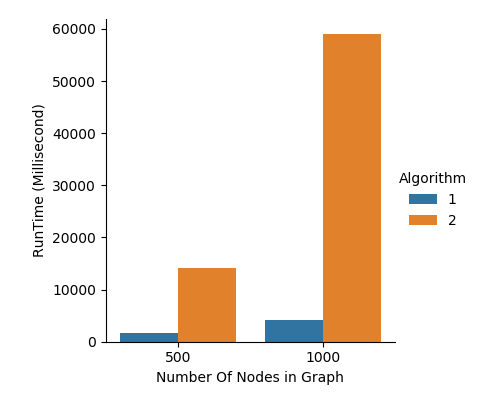
\includegraphics[scale = 0.7]{figure/figure.png}
	\caption{Time running in milliseconds of Algorithm 1 and 2 when the number of nodes in graph less than 500 and between 500 and 1000.}
	\label{figure_ASME} 
\end{figure}

\section{Conclusions}
In this article,we have presented Degree Centrality Algorithm and Betweenness Centrality Algorithm and we have also implemented these Algorithms and tested on our generated data set.

Although  Degree Centrality is more efficient than Betweenness Centrality, we use Degree Centrality in order to find popular users with a large number of followers and Betweenness Centrality quantifies the number of times a user acts as a bridge along the shortest path between two other users. In reality, the users were obtained from the Betweenness Centrality is more important. So, we were able to increase the effectiveness With the help of Betweenness Centrality.

Finally, it is expected that more research or even
a better understanding of the identifying influential users problem may lead to the emergence of more effective and efficient algorithms, as well as improvements in the Social Networks.\cite{art}

\bibliographystyle{asmems4}
\bibliography{asme2e}

\end{document}